%%%%%%%%%%%%%%%%%%%%%%%%%%%%%%%%%%%%%%%%%
% Journal Article
% LaTeX Template
% Version 1.4 (15/5/16)
%
% This template has been downloaded from:
% http://www.LaTeXTemplates.com
%
% Original author:
% Frits Wenneker (http://www.howtotex.com) with extensive modifications by
% Vel (vel@LaTeXTemplates.com)
%
% License:
% CC BY-NC-SA 3.0 (http://creativecommons.org/licenses/by-nc-sa/3.0/)
%
%%%%%%%%%%%%%%%%%%%%%%%%%%%%%%%%%%%%%%%%%

%----------------------------------------------------------------------------------------
%	PACKAGES AND OTHER DOCUMENT CONFIGURATIONS
%----------------------------------------------------------------------------------------

\documentclass[twoside,twocolumn]{article}

\usepackage{blindtext} % Package to generate dummy text throughout this template 

\usepackage[sc]{mathpazo} % Use the Palatino font
\usepackage[T1]{fontenc} % Use 8-bit encoding that has 256 glyphs
\linespread{1.05} % Line spacing - Palatino needs more space between lines
\usepackage{microtype} % Slightly tweak font spacing for aesthetics

\usepackage[english]{babel} % Language hyphenation and typographical rules

\usepackage[hmarginratio=1:1,top=32mm,columnsep=20pt]{geometry} % Document margins
\usepackage[hang, small,labelfont=bf,up,textfont=it,up]{caption} % Custom captions under/above floats in tables or figures
\usepackage{booktabs} % Horizontal rules in tables

\usepackage{lettrine} % The lettrine is the first enlarged letter at the beginning of the text

\usepackage{enumitem} % Customized lists
\setlist[itemize]{noitemsep} % Make itemize lists more compact

\usepackage{abstract} % Allows abstract customization
\renewcommand{\abstractnamefont}{\normalfont\bfseries} % Set the "Abstract" text to bold
\renewcommand{\abstracttextfont}{\normalfont\small\itshape} % Set the abstract itself to small italic text

\usepackage{titlesec} % Allows customization of titles
\renewcommand\thesection{\Roman{section}} % Roman numerals for the sections
\renewcommand\thesubsection{\roman{subsection}} % roman numerals for subsections
\titleformat{\section}[block]{\large\scshape\centering}{\thesection.}{1em}{} % Change the look of the section titles
\titleformat{\subsection}[block]{\large}{\thesubsection.}{1em}{} % Change the look of the section titles

\usepackage{fancyhdr} % Headers and footers
\pagestyle{fancy} % All pages have headers and footers
\fancyhead{} % Blank out the default header
\fancyfoot{} % Blank out the default footer
\fancyhead[C]{Running title $\bullet$ May 2016 $\bullet$ Vol. XXI, No. 1} % Custom header text
\fancyfoot[RO,LE]{\thepage} % Custom footer text

\usepackage{titling} % Customizing the title section

\usepackage{hyperref} % For hyperlinks in the PDF

\usepackage{graphicx} % For importing images
\usepackage{subfig}

%----------------------------------------------------------------------------------------
%	TITLE SECTION
%----------------------------------------------------------------------------------------

\setlength{\droptitle}{-4\baselineskip} % Move the title up

\pretitle{\begin{center}\Huge\bfseries} % Article title formatting
\posttitle{\end{center}} % Article title closing formatting
\title{Article Title} % Article title
\author{%
\textsc{Edric Tam}\\[1ex] % Your name
\normalsize Duke University \\ % Your institution
\normalsize \href{mailto:edric.tam@duke.edu}{edric.tam@duke.edu} % Your email address
\and % Uncomment if 2 authors are required, duplicate these 4 lines if more
\textsc{Craig Chen}\\[1ex] % Second author's name
\normalsize Duke University \\ % Second author's institution
\normalsize \href{mailto:craig.chen@duke.edu}{craig.chen@duke.edu} % Second author's email address
}
\date{\today} % Leave empty to omit a date
\renewcommand{\maketitlehookd}{%
\begin{abstract}
\noindent \blindtext % Dummy abstract text - replace \blindtext with your abstract text
\end{abstract}
}

%----------------------------------------------------------------------------------------

\begin{document}

% Print the title
\maketitle

%----------------------------------------------------------------------------------------
%	ARTICLE CONTENTS
%----------------------------------------------------------------------------------------

\section{Introduction}

\lettrine[nindent=0em,lines=3]{L} orem ipsum dolor sit amet, consectetur adipiscing elit.
\blindtext % Dummy text

\blindtext % Dummy text

%------------------------------------------------

\section{Preliminaries and Background}

\subsection{Generating Adversarial Images}
Maecenas sed ultricies felis. Sed imperdiet dictum arcu a egestas. 
\begin{itemize}
\item Donec dolor arcu, rutrum id molestie in, viverra sed diam
\item Curabitur feugiat
\item turpis sed auctor facilisis
\item arcu eros accumsan lorem, at posuere mi diam sit amet tortor
\item Fusce fermentum, mi sit amet euismod rutrum
\item sem lorem molestie diam, iaculis aliquet sapien tortor non nisi
\item Pellentesque bibendum pretium aliquet
\end{itemize}
\blindtext % Dummy text

Text requiring further explanation\footnote{Example footnote}.

\subsection{Persistent Homology}

%------------------------------------------------

\section{Methods}

\subsection{Adversarial Noise}
\blindtext % Dummy text

\subsection{Targeted Attacks}

%------------------------------------------------

\begin{figure*}[t!]
	\centering
	\subfloat[Mimic Image]{
	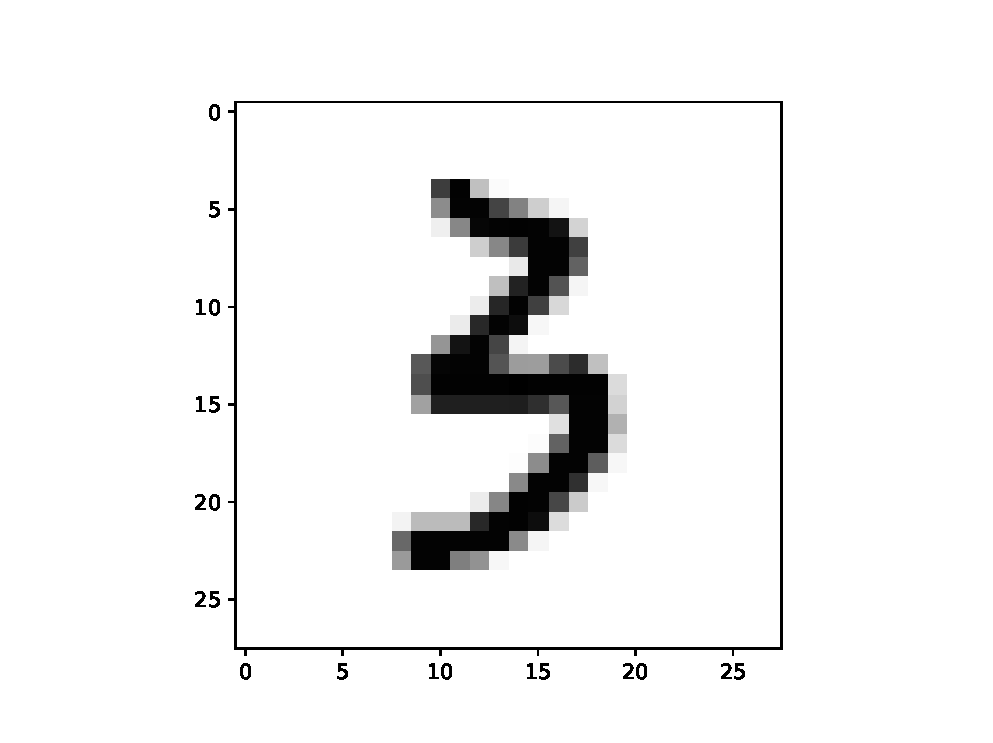
\includegraphics[scale=0.5]{figures/mimic3.eps}}
	\subfloat[Persistence Diagram of the mimic image]{
	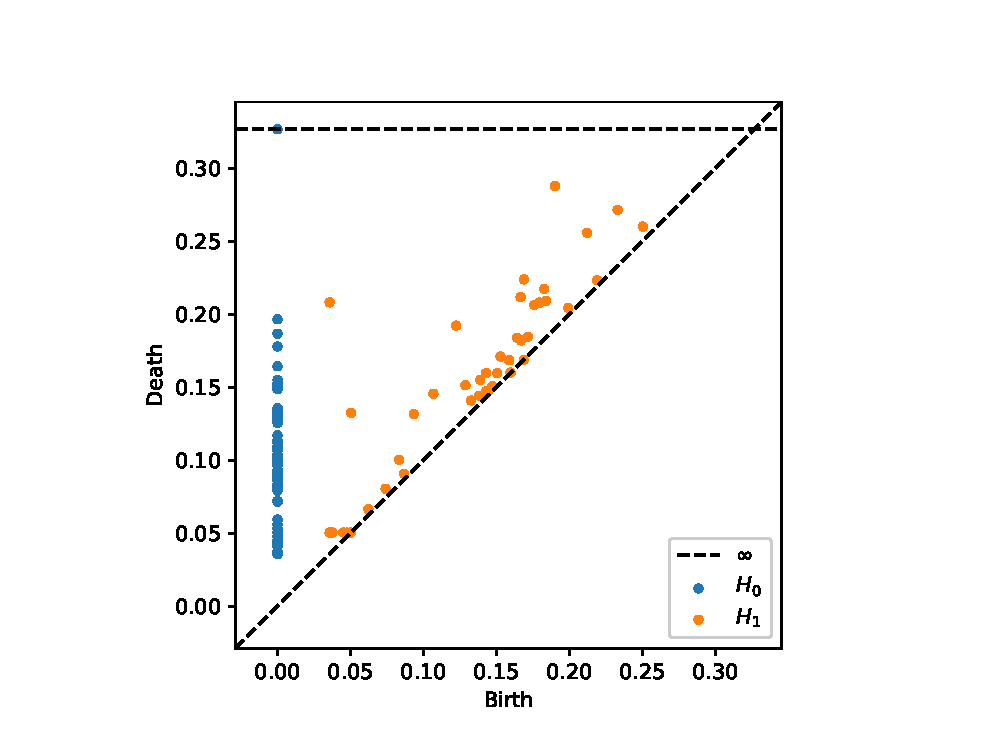
\includegraphics[scale=0.5]{figures/persdgm_mimic3.eps}}
	\\
	\subfloat[Adversarial Image, results in classification as 6]{
	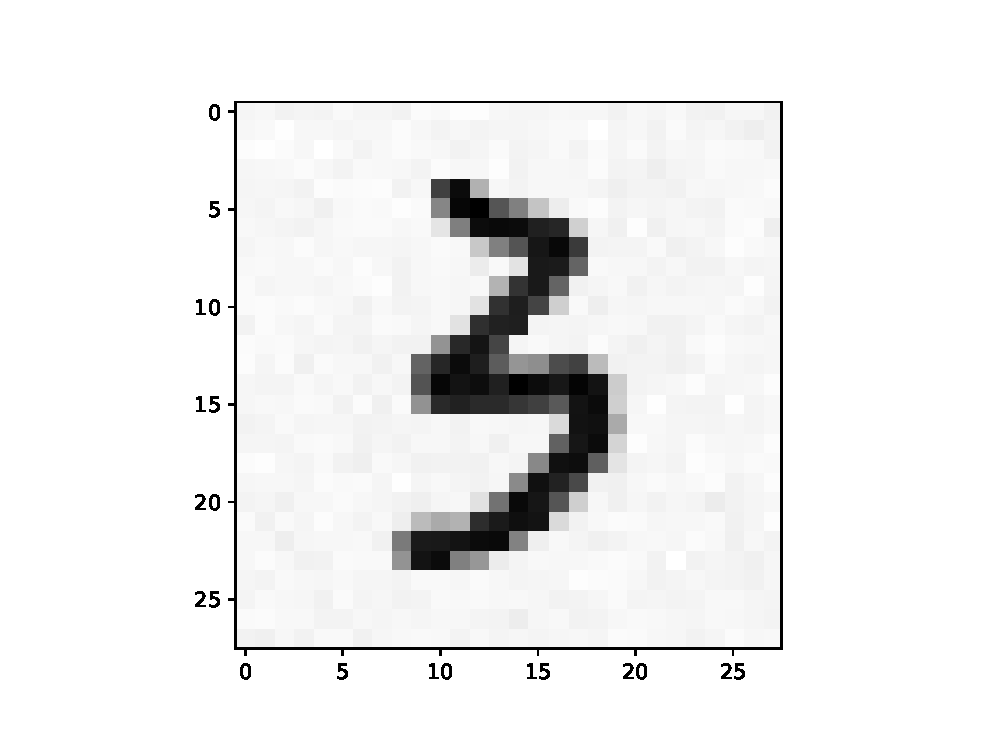
\includegraphics[scale=0.5]{figures/adversarial3.eps}}
	\subfloat[Persistence Diagram of the adversarial image]{
	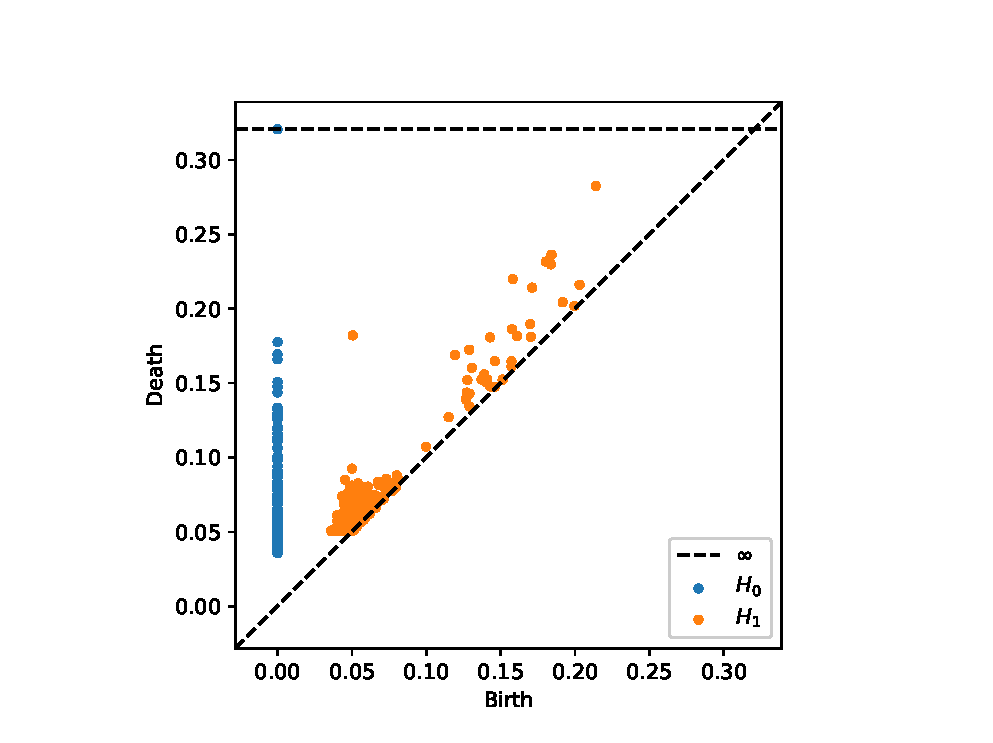
\includegraphics[scale=0.5]{figures/persdgm_adversarial3.eps}}
	\\
	\subfloat[$(\mu=0,\sigma^2=0.05)$ Gaussian Noise added]{
	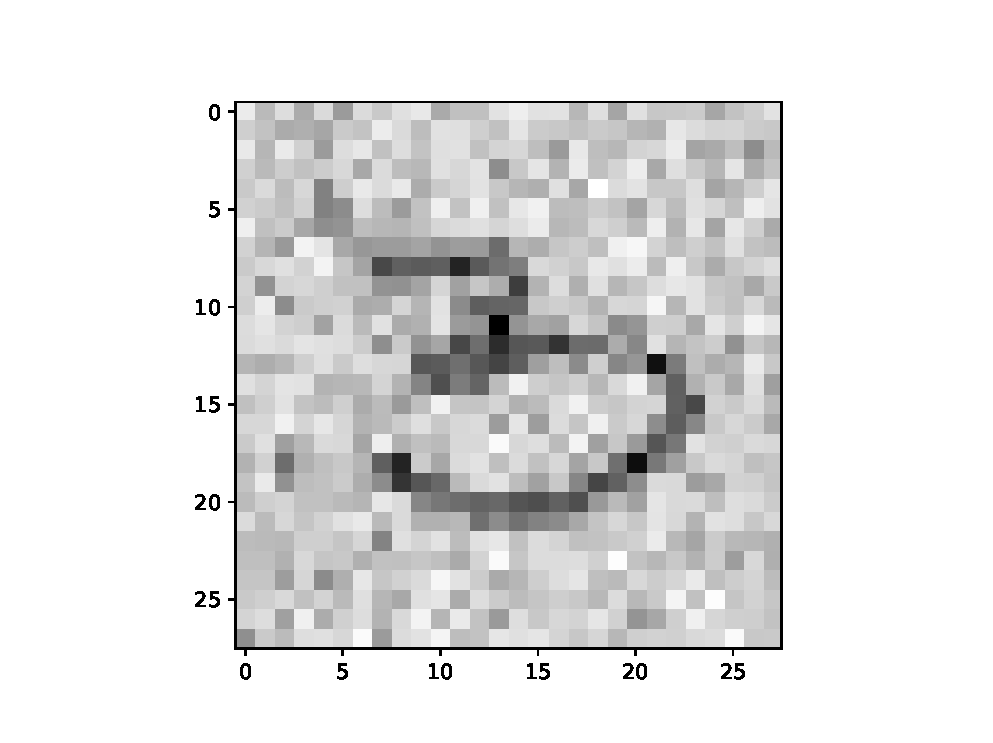
\includegraphics[scale=0.5]{figures/noisy3.eps}}
	\subfloat[Persistence Diagram of the noisy image]{
	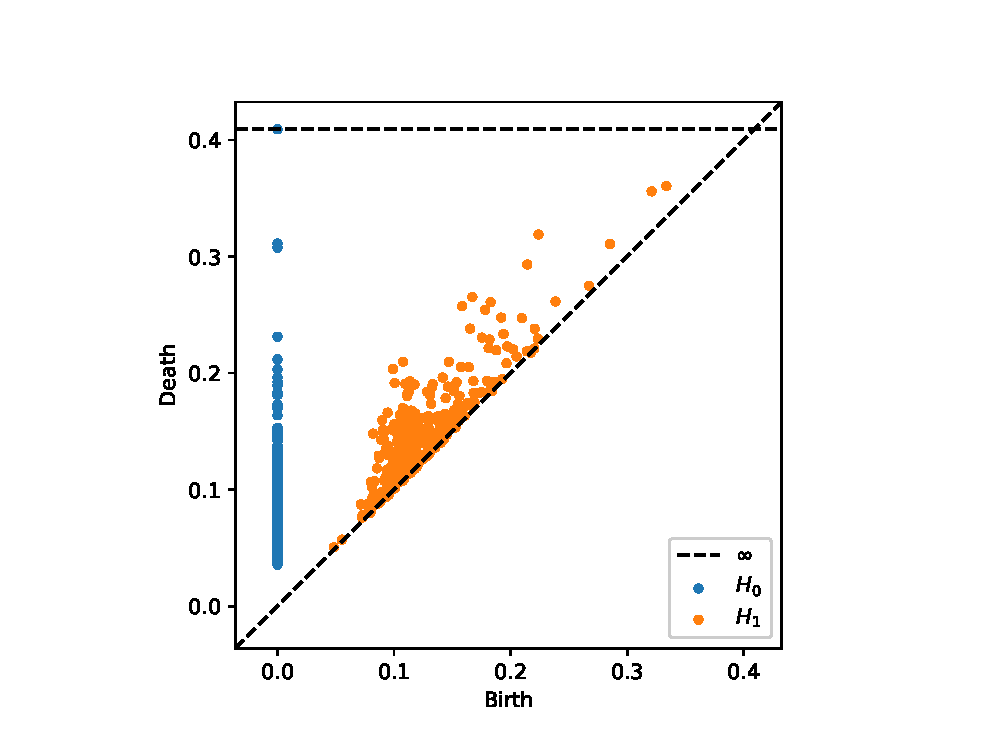
\includegraphics[scale=0.5]{figures/persdgm_noisy3.eps}}
	
	\caption{TEST}
\end{figure*}

\section{Results}



\blindtext % Dummy text

\begin{equation}
\label{eq:emc}
e = mc^2
\end{equation}

\blindtext % Dummy text

%------------------------------------------------

\section{Conclusion and Discussion}

\subsection{Subsection One}

A statement requiring citation \cite{Figueredo:2009dg}.
\blindtext % Dummy text

%----------------------------------------------------------------------------------------
%	REFERENCE LIST
%----------------------------------------------------------------------------------------

\begin{thebibliography}{99} % Bibliography - this is intentionally simple in this template

\bibitem[Figueredo and Wolf, 2009]{Figueredo:2009dg}
Figueredo, A.~J. and Wolf, P. S.~A. (2009).
\newblock Assortative pairing and life history strategy - a cross-cultural
  study.
\newblock {\em Human Nature}, 20:317--330.
 
\end{thebibliography}

%----------------------------------------------------------------------------------------

\end{document}
